%%%%%%%%%%%%%%%%%%%%%%%%%%%%%%%%%%%%%%%%%%%%%%%%%%%%%%%%%%%%%%%%%%%%%%
% Lớp 11 | Đường thẳng, mặt phẳng. Quan hệ song song trong | Điểm, đường thẳng và mặt phẳng
% Dạng 1H4?1-1: Câu hỏi lý thuyết
% Số câu: 47  (sinh tự động bởi tach_cau.py; từ nay thầy sửa trực tiếp file này)
%%%%%%%%%%%%%%%%%%%%%%%%%%%%%%%%%%%%%%%%%%%%%%%%%%%%%%%%%%%%%%%%%%%%%%

%%%%%%%%%%%%%%%% TRẮC NGHIỆM 4 PHƯƠNG ÁN %%%%%%%%%%%%%%%%

% nguồn: Ok_Toan11_TracNghiem_Lan2
\begin{ex}%[1H4N1-1]%[ma:2f7a6b40]
	Trong các tính chất sau, tính chất nào  không đúng?
	\choice{\True Có hai đường thẳng phân biệt cùng đi  qua hai điểm phân biệt cho trước}
		{Tồn tại 4  điểm không cùng thuộc một mặt phẳng}
		{Có một và chỉ một mặt phẳng đi qua ba  điểm không thẳng hàng}
		{Nếu một đường thẳng đi qua  hai điểm thuộc một mặt phẳng thì mọi điểm của đường thẳng đều thuộc mặt phẳng đó}
	 \loigiai{
	 Có hai đường thẳng phân biệt cùng đi qua hai điểm phân biệt cho trước là không đúng}
\end{ex}

% nguồn: Ok_Toan11_TracNghiem_Lan2
\begin{ex}%[1H4N1-1]%[ma:2735e699]
	Đường thẳng $ d$ nằm trong mặt  phẳng $(P)$ được kí hiệu là
	\choice 
		 {$ d\not\subset(P)$}
		{$ d\notin(P)$} 
		{\True  $ d\subset(P)$}
		 {$ d\in(P)$}
	 \loigiai{
	Đường thẳng $ d$  nằm trong mặt phẳng $(P)$ được kí hiệu là $ d\subset(P)$.}
\end{ex}

% nguồn: Ok_Toan11_TracNghiem_Lan2
\begin{ex}%[1H4N1-1]%[ma:5790094e]
	Cho tam giác $ABC$, gọi $M$ là điểm thuộc phần kéo dài của đoạn thẳng $BC$. Khẳng định nào sau đây  đúng?
	 \choice
		{\True  $M\in\left(ABC\right)$}
		 {$M\notin BC$}
		{$M\notin\left(ABC\right)$} 
		{$M\subset\left(ABC\right)$} 
	\loigiai{ 
	 \immini{
		Ta có $M\in BC\Rightarrow  M\in (ABC)$.
		} 
		{\begin{tikzpicture}[line join=round,line cap=round]
		 \coordinate (A) at (0,3);
		\coordinate (B) at (-2,0); 
		\coordinate  (C) at (3,0);
		\coordinate (M) at  ($(B)!3/2!(C)$);
		 \draw (A)--(B)--(C)--cycle (C)--(M);
		\foreach \i/\g in {A/90,B/-90,C/-90,M/-90}{\draw[fill=black](\i)  circle (1pt)
			($(\i)+(\g:3mm)$) node[scale=1]{$\i$};} 
	\end{tikzpicture}
		} 
	} 
\end{ex}

% nguồn: Ok_Toan11_TracNghiem_Lan2
\begin{ex}%[1H4N1-1]%[ma:3ce028e8]
	Điểm $  A$ thuộc mặt phẳng $(P)$ được kí hiệu là
	 \choice
		 {$ A\not\subset(P)$}
		{$  A\notin(P)$}
		{$ A\subset(P)$} 
		{\True $  A\in(P)$}
	\loigiai{ 
	Điểm $  A$ thuộc mặt phẳng $(P)$ được kí hiệu là $ A\in(P)$.}
\end{ex}

% nguồn: Ok_Toan11_TracNghiem_Lan2
\begin{ex}%[1H4N1-1]%[ma:5a3aa58a]
	Cho  biết mệnh đề nào sau đây là sai?
	\choice 
		{Qua ba điểm không thẳng hàng xác định duy nhất một mặt  phẳng}
		{Qua một đường thẳng và một điểm không  thuộc nó xác định duy nhất một mặt phẳng}
		{\True Qua ba điểm xác định duy nhất một mặt phẳng} 
		{Qua  hai đường thẳng cắt nhau xác định duy nhất một mặt phẳng}
	 \loigiai{
	Qua ba điểm không thẳng hàng xác định  duy nhất một mặt phẳng.}
\end{ex}

% nguồn: Ok_Toan11_TracNghiem_Lan2
\begin{ex}%[1H4N1-1]%[ma:aff70807]
	Hình chóp có $16$ cạnh thì có bao nhiêu mặt? 
	\choice{$10$} 
		{$8$} 
		{$7$} 
		{\True $9$} 
	\loigiai{ 
		 Hình chóp $S.{{A}_{1}}{{A}_{2}}\ldots{{A}_{n}}$, $\left( n\ge 3 \right)$ có $n$ cạnh bên và $n$ cạnh đáy nên có $2n$ cạnh.
		Ta  có: $2n=16\Leftrightarrow n=8$.
		Vậy khi đó hình chóp có $8$ mặt bên và $1$ mặt đáy nên nó có $9$ mặt. 
	 }
\end{ex}

% nguồn: Ok_Toan11_TracNghiem_Lan2
\begin{ex}%[1H4N1-1]%[ma:14684b28]
	Một mặt phẳng hoàn toàn được xác định nếu biết nó thoả  mãn điều kiện nào sau đây?
	 \choice
		 {Đi qua ba điểm bất kỳ}
		{Chứa  một đường thẳng và một điểm thuộc đường thẳng đó}
		{\True Chứa hai  đường thẳng cắt nhau}
		{Đi qua bốn điểm bất kỳ trong không gian} 
	 \loigiai{
	Một mặt phẳng  hoàn toàn được xác định nếu biết nó chứa hai đường thẳng cắt nhau.}
\end{ex}

% nguồn: Ok_Toan11_TracNghiem_Lan2
\begin{ex}%[1H4N1-1]%[ma:defbb7a2]
	Một hình  chóp có đáy là ngũ giác có số mặt và số cạnh là.
	 \choice{$5$ mặt, $5$ cạnh}
		{$6$ mặt, $5$  cạnh}
		{\True $6$ mặt, $10$  cạnh}
		{$5$ mặt, $10$  cạnh}
	 \loigiai{
		Hình chóp có  đáy là ngũ giác có:
		$6$ mặt gồm $5$ mặt bên và $1$ mặt đáy. 
		$10$ cạnh gồm  $5$ cạnh bên và $5$ cạnh đáy.
	 }
\end{ex}

% nguồn: Ok_Toan11_TracNghiem_Lan2
\begin{ex}%[1H4N1-1]%[ma:16779032]
	Các yếu tố nào sau đây  xác định một mặt phẳng duy nhất?
	 \choice
		{Ba điểm phân  biệt}
		{Một điểm và một đường  thẳng}
		{\True Hai  đường thẳng cắt nhau}
		 {Bốn điểm phân biệt}
	 \loigiai{
		Một mặt phẳng hoàn toàn xác định  khi cho hai đường thẳng cắt nhau.
	} 
\end{ex}

% nguồn: Ok_Toan11_TracNghiem_Lan2
\begin{ex}%[1H4N1-1]%[ma:907fa603]
	Một mặt phẳng hoàn toàn được xác định nếu biết điều nào sau đây? 
	\choice 
		{Một đường thẳng và một điểm thuộc  nó}
		{Ba điểm mà  nó đi qua}
		{\True Ba điểm  không thẳng hàng}
		{Hai đường  thẳng thuộc mặt phẳng}
	 \loigiai{Qua ba điểm không thẳng hàng xác định một và chỉ một mặt phẳng.}
\end{ex}

% nguồn: Ok_Toan11_TracNghiem_Lan2
\begin{ex}%[1H4N1-1]%[ma:9fbcab22]
	 Cho bốn điểm không đồng phẳng, ta có thể xác định được nhiều nhất bao nhiêu mặt phẳng phân biệt từ bốn điểm đã cho?
	 \choice
		{$3$} 
		{\True $4$} 
		{$2$} 
		{$6$} 
	 \loigiai{
	Do bốn điểm không đồng phẳng nên không tồn tại bộ ba điểm thẳng hàng trong số bốn điểm đó. Cứ  ba điểm không thẳng hàng xác định một mặt phẳng nên số mặt phẳng phân biệt có thể lập được từ bốn điểm đã cho là $\mathrm{C}_4^3=4$.}
\end{ex}

% nguồn: Ok_Toan11_TracNghiem_Lan2
\begin{ex}%[1H4N1-1]%[ma:07895e01]
	\immini{ 
	Cho hình chóp $S.ABCDE$, số mặt của hình chóp  đó là bao nhiêu?
	\choice 
		{$4$} 
		{$7$} 
		{$5$} 
		{\True  $6$}
		} 
		{\begin{tikzpicture}[line join=round,line cap=round]
		\coordinate (S) at (1,4); 
		\coordinate (A) at  (0,0);
		\coordinate (B) at  (1,-2);
		\coordinate  (C) at (3,-3);
		 \coordinate (E) at (5,0);
		\coordinate (D) at  (4,-2);
		\draw  (S)--(A)
			(S)--(B) 
			 (S)--(C)
			 (S)--(D)
			 (S)--(E)
			 (A)--(B)--(C)--(D)--(E);
		 \draw[dashed,thin](A)--(E);
		\foreach \i/\g in {S/90,A/180,B/-90,C/-90,D/-30,E/0}{\draw[fill=black](\i) circle  (1pt)
			($(\i)+(\g:3mm)$) node[scale=1]{$\i$};} 
	\end{tikzpicture}
		} 
	 \loigiai{
	 Hình chóp $S.ABCDE$ có 6 mặt.}
\end{ex}

% nguồn: Ok_Toan11_TracNghiem_Lan2
\begin{ex}%[1H4N1-1]%[ma:0b54fcdc]
	Trong không gian cho bốn điểm không đồng phẳng, có thể xác định nhiều nhất bao nhiêu mặt phẳng phân biệt  từ các điểm đó?
	 \choice{$3$}
		{\True  $4$}
		 {$2$}
		{$6$} 
	\loigiai{ 
		Trong không gian, bốn điểm không đồng phẳng tạo thành một hình tứ diện. Vì vậy xác  định nhiều nhất bốn mặt phẳng phân biệt.
	} 
\end{ex}

% nguồn: Ok_Toan11_TracNghiem_Lan2
\begin{ex}%[1H4N1-1]%[ma:6ea64a68]
	Cho hình chóp $S.ABC$. Gọi $M$, $N$, $K$, $E$ lần lượt là trung điểm của $SA$, $SB$, $SC$, $BC$. Bốn điểm nào sau đây  đồng phẳng?
	\choice{\True  $M,K,A,C$}
		{$M,N,A,C$} 
		{$M,N,K,C$} 
		 {$M,N,K,E$}
	\loigiai{ 
		\begin{center}
			\begin{tikzpicture}[scale=1.5,font=\small,line join=round,line cap=round,>=stealth]
					\path 
						(0,0)  coordinate (A)
						($(A)+(1,-1)$)  coordinate (C)
						($(A)+(3,0)$) coordinate (B) 
						 ($(A)+(1,2)$) coordinate (S)
						($(S)!0.5!(A)$) coordinate (M) 
						($(S)!0.5!(B)$) coordinate  (N)
						($(S)!0.5!(C)$) coordinate  (K)
						 ($(B)!0.5!(C)$) coordinate (E);
					\draw  (S)--(A)--(C)--(B)--(S)--(C);
					\draw[dashed] (A)--(B); 
					\foreach \x/\g in  {A/180,B/0,C/-90,S/90,N/45,K/-150,M/-180,E/-30}
					\fill (\x) circle (1pt) 
						 ($(\g:3mm)+(\x)$) node {$\x$};
				\end{tikzpicture}
		\end{center}
		Ta thấy $M,K$ cùng thuộc mặt phẳng $\left( SAC  \right)$ nên bốn điểm $M$; $K$; $A$; $C$ đồng phẳng.
	 }
\end{ex}

% nguồn: Ok_Toan11_TracNghiem_Lan2
\begin{ex}%[1H4N1-1]%[ma:93304db8]
	Trong các mệnh đề sau, mệnh đề nào sau  đây {\bf sai}?
	\choice 
		{Trong  không gian, hai đường thẳng phân biệt cùng song song với đường thẳng thứ ba thì song song với nhau}
		{Nếu ba mặt phẳng đôi một cắt nhau  theo ba giao tuyến phân biệt thì ba giao tuyến đó đồng quy hoặc đôi một song song với nhau}
		{Nếu hai mặt phẳng phân biệt lần lượt chứa hai đường thẳng song song với nhau thì giao tuyến của  chúng song song với hai đường thẳng đó hoặc trùng với một trong hai đường thẳng đó}
		{\True Trong không gian, qua một điểm và một đường  thẳng cho trước, có đúng một đường thẳng song song với đường thẳng đã cho}
	 \loigiai{
	Trong không gian, qua một điểm không nằm trên một đường thẳng cho trước,  có đúng một đường thẳng song song với đường thẳng đã cho.}
\end{ex}

% nguồn: Ok_Toan11_TracNghiem_Lan2
\begin{ex}%[1H4N1-1]%[ma:1326cdf3]
	Cho hai đường thẳng $a$ và $b$ chéo nhau. Có bao nhiêu mặt phẳng chứa $a$ và song  song với $b$.
	 \choice{$0$}
		 {Vô số}
		{$2$} 
		{\True $1$} 
	 \loigiai{
	Trong không gian hai đường thẳng  $a$ và $b$ chéo nhau, có một và chỉ một mặt phẳng đi qua $a$ và song song với $b$.}
\end{ex}

% nguồn: Ok_Toan11_TracNghiem_Lan2
\begin{ex}%[1H4N1-1]%[ma:bff62158]
	Một hình  chóp có đáy là ngũ giác có số cạnh là.
	\choice{$9$ cạnh} 
		{\True  $10$ cạnh}
		{$6$ cạnh} 
		 {$5$ cạnh}
	\loigiai{ 
		Hình chóp có số cạnh bên bằng số cạnh đáy nên số cạnh  của hình chóp là: $5+5=10$.
	 }
\end{ex}

% nguồn: Ok_Toan11_TracNghiem_Lan2
\begin{ex}%[1H4N1-1]%[ma:f2c2e078]
	Trong các mệnh đề sau, mệnh  đề nào đúng?
	\choice{Hai đường thẳng phân biệt không song song thì cheo  nhau}
		 {Hai đường thẳng không có điểm chung thì chéo nhau}
		{\True Hai đường thẳng chéo nhau thì không  có điểm chung}
		{Hai đường thẳng lần lượt nằm trên hai mặt phẳng phân  biệt thì chéo nhau}
	\loigiai{ 
	hai đường thẳng  chéo nhau là hai đường thẳng không cùng nằm trong mặt phẳng nên chúng không có điểm chung}
\end{ex}

% nguồn: Ok_Toan11_TracNghiem_Lan2
\begin{ex}%[1H4N1-1]%[ma:a10780ae]
	Cho điểm $A$ thuộc mặt phẳng  $(P)$, cách viết nào dưới đây là đúng
	\choice 
		 {$(P)\in A$}
		{$A\notin(P)$} 
		 {$A\subset(P)$}
		{\True $A\in(P)$} 
	 \loigiai{
		 Ta có $A\in(P)$.
	 }
\end{ex}

% nguồn: Ok_TracNghiemLop11_Lan1
\begin{ex}%[1H4N1-1]%[ma:e39829d6]
	\immini[thm]{Cho hình chóp $S.ABCD$ như hình vẽ. Hỏi hình chóp đó có  bao nhiêu mặt phẳng?
	 \choice
		 {$4$}
		{\True  $5$}
		{$1$} 
		{$8$} 
		}{ 
		\begin{tikzpicture}[line join=round,line cap=round,scale=0.5]
				 \tikzset{every node/.style={scale=0.7}}
				\coordinate (S)  at (1,4);
				\coordinate (A)  at (0,0);
				 \coordinate (B) at (1,-2);
				\coordinate  (C) at (3,-3);
				\coordinate (D)  at (5,0);
				 \draw (S)--(A)
					(S)--(B) 
					 (S)--(C)
					(S)--(D) 
					 (B)--(C)
					 (A)--(B)--(C)--(D);
				\draw[dashed](A)--(D); 
				\foreach \i/\g  in {S/90,A/180,B/-100,C/-90,D/0}{\draw[fill](\i) circle (1pt)
					($(\i)+(\g:3.5mm)$)  node[scale=1]{$\i$};}
			\end{tikzpicture}
		} 
	 \loigiai{
		Dựa vào hình vẽ ta thấy hình chóp có $4$ mặt bên và $1$ mặt đáy. 
	} 
\end{ex}

% nguồn: Ok_TracNghiemLop11_Lan1
\begin{ex}%[1H4N1-1]%[ma:3cd025c5]
	 Trong không gian, mệnh đề nào sau đây là đúng?
	 \choice
		{Qua bốn điểm phân biệt xác định một  mặt phẳng duy nhất}
		 {\True Qua ba điểm phân biệt không thẳng hàng xác định một mặt phẳng duy nhất}
		{Qua một điểm  và một đường thẳng xác định một mặt phẳng duy nhất}
		{Qua hai đường thẳng bất kì  xác định một mặt phẳng duy nhất}
	\loigiai{ 
	Mệnh đề đúng là qua ba điểm phân biệt không thẳng hàng xác định  một mặt phẳng duy nhất.}
\end{ex}

% nguồn: Ok_TracNghiemLop11_Lan1
\begin{ex}%[1H4N1-1]%[ma:727f07b6]
	 Trong các khẳng định sau, khẳng định nào đúng?
	\choice 
		{Qua  $2$ điểm phân biệt có duy nhất một mặt phẳng}
		{Qua $3$ điểm  phân biệt bất kì có duy nhất một mặt phẳng}
		{\True Qua $3$ điểm không thẳng hàng có duy nhất một mặt  phẳng}
		{Qua $4$ điểm phân biệt bất kì có duy nhất một mặt  phẳng}
	 \loigiai{
		\lq\lq Qua $3$ điểm  không thẳng hàng có duy nhất một mặt phẳng\rq\rq \, là khẳng định đúng.
	} 
\end{ex}

% nguồn: Ok_TracNghiemLop11_Lan1
\begin{ex}%[1H4N1-1]%[ma:f7dffbef]
	Cho tứ giác $ABCD$. Có bao nhiêu mặt  phẳng chứa các đỉnh của tứ giác $ABCD$?
	 \choice
		{vô số} 
		 {$4$}
		{$2$} 
		 {\True $1$}
	 \loigiai{
		Có duy nhất  một mặt phẳng chứa các đỉnh của tứ giác $ABCD$.
	} 
\end{ex}

% nguồn: Ok_TracNghiemLop11_Lan1
\begin{ex}%[1H4N1-1]%[ma:3fcc76e5]
	Cho tam giác $ABC$  và $M$ là trung điểm của $AB$. Khẳng định nào sau đây đúng?
	 \choice
		{  $A\subset\left(ABC\right)$}
		{\True  $M\in \left(ABC\right)$}
		{ $AB\in \left(ABC\right)$} 
		 {$C\notin\left(ABC\right)$}
	 \loigiai{
		$M$ là  trung điểm của $AB \Rightarrow M \in AB$.\\
		Mà $AB \subset (ABC) \Rightarrow M \in (ABC)$. 
	} 
\end{ex}

% nguồn: Ok_TracNghiemLop11_Lan1
\begin{ex}%[1H4N1-1]%[ma:8b087a27]
	 \immini{
	Cho đường thẳng $a$ đi qua hai điểm phân biệt $M$, $N$  và điểm $O$ không thuộc $a$. Có bao nhiêu mặt phẳng đi qua ba điểm $M$, $N$, $O$?
	\choice[2] 
		 {\True $1$}
		 {$2$}
		{$3$} 
		 {Vô số}
		}{ 
		\begin{tikzpicture}[font=\footnotesize]
				\path  (0,0) coordinate (M)
					(2,.7) coordinate  (N)
					 (.8,1.4) coordinate (O);
				\draw[shorten <=-.7 cm,shorten >=-1 cm] (M)--(N); 
				\foreach \t/\g in {M/90,N/90,O/90}{ 
					\draw[fill] (\t)  circle (1pt) node[shift={(\g:7pt)}]{$\t$};
				} 
				\path  ($(M)!1.3!(N)$) node[below]{$a$};
			\end{tikzpicture}
		 }
	 \loigiai{
		Do $O$ không thuộc $a$ nên ba điểm $M$, $N$, $O$ không thẳng hàng. Do đó chỉ có  một mặt phẳng đi qua ba điểm $M$, $N$, $O$.
	} 
\end{ex}

% nguồn: Ok_TracNghiemLop11_Lan1
\begin{ex}%[1H4N1-1]%[ma:c1ff94db]
	Trên mặt phẳng cho $4$ điểm $A$,  $B$, $C$, $D$ như hình vẽ. Ba điểm nào dưới đây không xác định một mặt phẳng?
	\begin{center}
		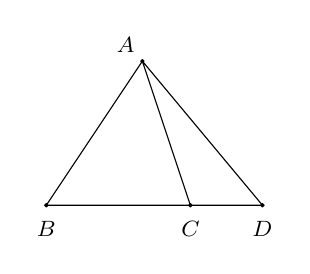
\begin{tikzpicture}[>=stealth,line join=round,line cap=round,font=\footnotesize,scale=.61]
				 \path
					(0,0) coordinate  (B)
					(3,0) coordinate (C) 
					 (4.5,0) coordinate (D)
					 (2,3) coordinate (A);
				 \draw (A)--(B)--(D)--(A)
					(A)--(C); 
				\foreach \p/\g  in {B/-90,C/-90,D/-90,A/135}
				\draw[fill] (\p) circle (1pt) node[shift=(\g:3mm)]  {$\p$};
			\end{tikzpicture}
	\end{center}
	 \choice
		{$A$, $B$,  $C$}
		{\True $B$, $C$,  $D$}
		 {$A$, $B$, $D$}
		{$A$, $C$,  $D$}
	\loigiai{Vì $B$, $C$, $D$ thẳng hàng nên không xác  định $1$ mặt phẳng.}
\end{ex}

% nguồn: Ok_TracNghiemLop11_Lan1
\begin{ex}%[1H4N1-1]%[ma:3d73b9be]
	Trong mặt phẳng $\left( \alpha \right)$, cho bốn điểm $A$, $B$, $C$, $D$ trong đó không có ba điểm nào thẳng hàng. Điểm $S\notin \left( \alpha \right)$.  Có bao nhiêu mặt phẳng tạo bởi $S$ và hai trong bốn điểm nói trên?
	 \choice
		 {$4$}
		 {$5$}
		 {\True $6$}
		 {$8$}
	\loigiai{ 
	Qua $3$ điểm phân biệt không thẳng hàng thì chỉ xác định duy nhất $1$ và chỉ $1$ mặt phẳng.  \\
	Chọn  $2$ điểm trong $4$ điểm có $\mathrm{C}_{4}^{2}$. Vậy số mặt phẳng cần tìm là $\mathrm{C}_{4}^{2}=6$.
	} 
\end{ex}

% nguồn: Ok_TracNghiemLop11_Lan1
\begin{ex}%[1H4N1-1]%[ma:4d395e0a]
	Trong không gian, cho tứ diện $ABCD$. Có thể xác định được bao nhiêu mặt phẳng phân biệt từ $3$  trong số $4$ đỉnh của tứ diện đã cho?
	\choice 
		 {\True $4$}
		{$3$} 
		{$2$} 
		 {$6$}
	 \loigiai{
		\begin{center}
			\begin{tikzpicture}[scale=1,font=\footnotesize,line join=round,line cap=round,>=stealth]
					\coordinate  (B) at (0,0);
					 \coordinate (C) at (1.3,-1.7);
					 \coordinate (D) at (4,0);
					\coordinate (A)  at (2.7,3.5);
					\draw  (A)--(B)--(C)--(D)--(A)--(C);
					\draw[dashed] (B)--(D); 
					\foreach  \x/\g in{A/90,B/180,C/-90,D/0} \fill (\x) circle (1pt)+(\g:.35) node{$\x$};
				\end{tikzpicture}
		\end{center}
	Có $4$ mặt phẳng phân biệt được tạo từ $3$ trong số $4$ đỉnh của tứ diện đã cho là các mặt phẳng $(ABC)$; $(BCD)$;  $(ACD)$; $(ABD)$.}
\end{ex}

% nguồn: Ok_Toan11_TracNghiem_Lan2
\begin{ex}%[1H4H1-1]%[ma:7a0a3e2d]
	Cho hình chóp $S.ABC$. Gọi $M$, $N$, $K$, $E$ lần lượt là trung điểm của $SA$, $SB$, $SC$, $BC$. Bốn điểm nào sau  đây đồng phẳng?
	 \choice
		 {\True $M$, $K$, $A$, $C$}
		{$M$, $N$, $A$,  $C$}
		{$M$,  $N$, $K$, $C$}
		 {$M$, $N$, $K$, $E$}
	\loigiai{ 
	 \immini
		{Ta thấy $M$,  $K$ cùng thuộc mặt phẳng $(SAC)$ nên bốn điểm $M$, $K$, $A$, $C$ đồng phẳng.}
		{\begin{tikzpicture}[scale=1,font=\footnotesize,line join=round,line cap=round,>=stealth]
		\path (0,0) coordinate  (A)
			 (3,0) coordinate (B)
			(-30:2.5) coordinate (C) 
			(70:2) coordinate (S) 
			 ($(S)!1/2!(A)$) coordinate (M)
			($(S)!1/2!(B)$) coordinate  (N)
			 ($(S)!1/2!(C)$) coordinate (K)
			 ($(B)!1/2!(C)$) coordinate (E);
		\draw (S)--(A)--(C)--(B)--cycle (C)--(S) 
			(M)--(K); 
		\draw[dashed]  (A)--(B);
		\foreach \x/\g in  {S/90,A/180,C/-90,B/0,M/180,N/0,K/45,E/-45}{
			\fill  (\x) circle (1pt)+(\g:0.3) node{$\x$};
		} 
	\end{tikzpicture}
		} 
	 }
\end{ex}

% nguồn: Ok_Toan11_TracNghiem_Lan2
\begin{ex}%[1H4H1-1]%[ma:84da2a7f]
	Hình vẽ  nào sau đây biểu diễn hình chóp tứ giác?
	\choice 
		{\begin{tikzpicture}[line join=round,line cap=round,scale=.6]
		\coordinate (A)  at (0,0);
		\coordinate (B) at  (3,-2);
		\coordinate (D) at (5,0); 
		\coordinate (C) at  ($(B)+(D)-(A)$);
		\coordinate  (O) at ($(A)!0.5!(C)$);
		\coordinate (S)  at ($(O)+(0,4)$);
		\coordinate (M) at ($(S)!2!(O)$); 
		 \draw (S)--(A)
			 (S)--(B)
			 (S)--(C)
			 (A)--(B)
			(B)--(C) 
			(M)--(B) 
			(M)--(C) 
			 (M)--(A);
		\draw[dashed,thin](A)--(D) 
			 (C)--(D)
			(S)--(D) 
			 (M)--(D);
		 \foreach \i/\g in {S/90,A/180,B/-90,C/-90,D/0,M/-90}{\draw[fill=black](\i) circle (1pt)
			 ($(\i)+(\g:3mm)$);}
	\end{tikzpicture}
		} 
		{\begin{tikzpicture}[line join = round,line cap = round,>=stealth,scale=.6]
		\coordinate (A) at  (0,0);
		\coordinate (B) at  (2,-2);
		\coordinate (C) at  (5,0);
		\coordinate (A') at ($(A)+(0,5)$); 
		 \coordinate (B') at ($(A')+(B)-(A)$);
		 \coordinate (C') at ($(A')+(C)-(A)$);
		 \draw (A')--(B')--(C')--cycle (A')--(A)--(B)--(C)--(C')
			 (B)--(B');
		\draw[dashed,thin](A)--(C); 
		\foreach \i/\g in {A/180,A'/180,B/-90,C/-90,B'/0,C'/-90}{\draw[fill=black](\i) circle (1pt) 
			 ($(\i)+(\g:3mm)$);}
	\end{tikzpicture}
		} 
		{\begin{tikzpicture}[line join=round,line cap=round,scale=.6]
		\coordinate (A)  at (-2,0);
		\coordinate (B)  at (0,-3);
		\coordinate (C)  at (3,0);
		\coordinate (S) at ($(A)+(0,4)$); 
		 \draw (S)--(A)
			 (S)--(B)
			 (S)--(C)
			 (B)--(C)
			(A)--(B); 
		 \draw[dashed,thin](A)--(C);
		 \foreach \i/\g in {S/90,A/180,B/-90,C/0}{\draw[fill=black](\i) circle (1pt)
			($(\i)+(\g:3mm)$);} 
	\end{tikzpicture}
		} 
		{\True \begin{tikzpicture}[line join=round,line cap=round,scale=.6]
		\coordinate (A) at  (0,0);
		\coordinate  (B) at (-2,-3);
		\coordinate  (D) at (7,0);
		\coordinate  (C) at ($(B)+(D)-(A)$);
		\coordinate  (S) at ($(A)+(0,5)$);
		\draw (S)--(B) 
			 (S)--(C)
			(S)--(D) 
			(B)--(C)--(D); 
		 \draw[dashed,thin](S)--(A)
			(A)--(B) 
			 (A)--(D);
		\foreach \i/\g in {S/90,A/-90,B/-90,C/-90,D/0}{\draw[fill=black](\i) circle (1pt) 
			($(\i)+(\g:3mm)$);} 
	\end{tikzpicture}
		} 
	 \loigiai{
	Hình D biểu diễn hình chóp tứ giác.} 
\end{ex}

% nguồn: Ok_Toan11_TracNghiem_Lan2
\begin{ex}%[1H4H1-1]%[ma:8a099bad]
	Cho bốn điểm $A,\,B,\,C,\,D$ không cùng nằm trong một mặt phẳng. Trên $AB$, $AD$ lần lượt lấy các điểm $M$  và $N$ sao cho $MN$ cắt $BD$ tại $I$. Điểm $I$ không thuộc mặt phẳng nào sao đây?
	 \choice
		{$\left(BCD\right)$} 
		{$\left(ABD\right)$} 
		{$\left(CMN\right)$} 
		 {\True $\left(ACD\right)$}
	 \loigiai{
	 \immini{
		Ta có $I\in BD\Rightarrow I\in\left(BCD\right)$ và  $I\in\left(ABD\right)$.\\
		$I\in MN\Rightarrow  I\in\left(CMN\right)$.}
		{\begin{tikzpicture}[line join=round,line cap=round]
		\coordinate (A) at  (0,4);
		\coordinate (B) at  (-2,0);
		\coordinate (C) at  (0,-3);
		\coordinate (D) at (3,0); 
		\coordinate (M) at  ($(A)!1/3!(B)$);
		\coordinate  (N) at ($(A)!2/3!(D)$);
		 \coordinate (I) at (intersection of B--D and M--N);
		\draw  (A)--(B)
			 (A)--(C)
			(A)--(D) 
			 (C)--(D)
			 (B)--(C)
			 (D)--(I)--(N);
		 \draw[dashed,thin](B)--(D)
			(M)--(N); 
		\foreach \i/\g in {A/90,B/180,C/-90,D/-90,M/-180,N/-120,I/-90}{\draw[fill=black](\i)  circle (1pt)
			($(\i)+(\g:3mm)$)  node[scale=1]{$\i$};}
	\end{tikzpicture}
		 }
	 }
\end{ex}

% nguồn: Ok_Toan11_TracNghiem_Lan2
\begin{ex}%[1H4H1-1]%[ma:6df671f7]
	 Cho tam giác $ABC$, lấy điểm $I$ trên cạnh $AC$ kéo dài. Mệnh đề nào sau đây \textbf{sai}?
	 \choice
		{$A\in  (ABC)$}
		 {$I\in (ABC)$}
		{$(ABC)\equiv (IBC)$} 
		{\True $BI\not\subset  (ABC)$}
	\loigiai{ 
	\immini 
		{Ta có điểm $I\in AC\subset(ABC)$  nên $BI\subset (ABC)$. Vậy $BI\not\subset (ABC)$ là mệnh đề sai.}
		{\begin{tikzpicture}[scale=1,font=\footnotesize,line join=round,line cap=round,>=stealth]
		\path  (0,0) coordinate (A)
			(60:1.5) coordinate  (B)
			(1.5,0)  coordinate (C)
			(3,0)  coordinate (I);
		\draw  (C)--(B)--(A)--(I);
		\foreach \x/\g in {A/180,B/90,C/45,I/0}{\fill (\x) circle (1pt)+(\g:0.3) node{$\x$};} 
	\end{tikzpicture}
		 }
	 }
\end{ex}

% nguồn: Ok_Toan11_TracNghiem_Lan2
\begin{ex}%[1H4H1-1]%[ma:10569745]
	Cho bốn điểm $A$ ,$B$  ,$C$ ,$D$ không đồng phẳng, ta có thể xác định được nhiều nhất bao nhiêu mặt phẳng phân biệt từ bốn điểm đã cho?
	 \choice
		 {$2$}
		 {$3$}
		{\True  $4$}
		{$6$} 
	 \loigiai{
	 \immini{
		Cứ ba điểm không  thẳng hàng thì sẽ cho ta một mặt phẳng.\\
		Vì vậy, từ bốn điểm $A$, $B$, $C$, $D$  không đồng phẳng ta có các mặt phẳng sau $\left(ABC\right);\,\left(ABD\right);\,\left(BCD\right);\,\left(ACD\right).$}
		{\begin{tikzpicture}[line join=round,line cap=round,scale=.7]
		\coordinate (A) at  (0,4);
		\coordinate (B) at (-2,0); 
		 \coordinate (C) at (0,-3);
		\coordinate  (D) at (3,0);
		\draw (A)--(B) 
			(A)--(C) 
			(A)--(D) 
			(C)--(D) 
			 (B)--(C);
		 \draw[dashed,thin](B)--(D);
		\foreach \i/\g in {A/90,B/180,C/-90,D/0}{\draw[fill=black](\i) circle  (1pt)
			($(\i)+(\g:3mm)$) node[scale=1]{$\i$};} 
	\end{tikzpicture}
		} 
	} 
\end{ex}

% nguồn: Ok_Toan11_TracNghiem_Lan2
\begin{ex}%[1H4H1-1]%[ma:e279032b]
	Cho tứ diện $ ABCD$, $ M$ là trung  điểm $ CD$. Chọn khẳng định đúng?
	 \choice
		{$  AM\subset\left(ABC\right)$}
		 {$ AM\subset\left(ABD\right)$}
		{\True $ AM\subset\left(ACD\right)$} 
		 {$ AM\subset\left(BCD\right)$}
	\loigiai{ 
	 \immini{Có $ A\in\left(ACD\right)$ và $ M\in CD\subset\left(ACD\right)$ nên $ AM\subset\left(ACD\right)$.}{
		\begin{tikzpicture}[line join=round,line cap=round,line width=.6pt,font=\footnotesize,scale=1]
				\coordinate[label=left:$B$] (B) at  (0,0);
				\coordinate[label=below  left:$C$] (C) at (1,-1);
				 \coordinate[label=right:$D$] (D) at (4,0);
				\coordinate[label=below right:$M$] (M) at  ($(C)!.5!(D)$);
				\coordinate (O) at  ($(B)!2/3!(M)$);
				\coordinate[label=above  left:$A$] (A) at ($(O)+(90:4)$);
				\draw (A)--(B)--(C)--(D)--cycle  (M)--(A)--(C);
				\draw[dashed] (B)--(D); 
				\fill (A) circle  (1pt)
					 (B) circle (1pt)
					(C) circle  (1pt)
					 (D) circle (1pt)
					(M) circle  (1pt);
			\end{tikzpicture}
		 }
	} 
\end{ex}

% nguồn: Ok_Toan11_TracNghiem_Lan2
\begin{ex}%[1H4H1-1]%[ma:6e0b47ee]
	Cho hình chóp tứ giác $S.ABCD$ có đáy $ABCD$ là hình bình hành tâm $O$. Điểm $M$ thuộc cạnh $SO$  ($M$ khác $S$ và $M$ khác $O$). Trong các mặt phẳng sau, điểm $M$ nằm trên mặt phẳng nào?
	\choice 
		 {$\left(ABCD\right)$}
		{\True  $\left(SBD\right)$}
		{$\left(SAB\right)$} 
		{$\left(SCD\right)$} 
	 \loigiai{
	\immini{ 
		 Ta có $M\in SO$ và $SO\subset\left(SBD\right)\Rightarrow M\in\left(SBD\right)$.}
		{\begin{tikzpicture}[line join=round,line cap=round,scale=.7]
		\coordinate (A) at  (0,0);
		\coordinate (B)  at (2,-2);
		\coordinate  (D) at (5,0);
		\coordinate (C) at ($(B)+(D)-(A)$); 
		\coordinate  (O) at ($(A)!0.5!(C)$);
		\coordinate (S) at ($(O)+(-1,6)$); 
		\coordinate (M) at ($(S)!2/3!(O)$); 
		\draw  (S)--(A)
			 (S)--(B)
			 (S)--(C)
			 (A)--(B)
			 (B)--(C);
		 \draw[dashed,thin](A)--(C)
			 (A)--(D)
			(C)--(D) 
			 (S)--(D)
			(S)--(O) 
			 (B)--(D);
		\foreach \i/\g in  {S/90,A/180,B/-90,C/-90,D/20,O/-90,M/ 0}{\draw[fill=black](\i) circle (1pt)
			($(\i)+(\g:3mm)$)  node[scale=1]{$\i$};}
	\end{tikzpicture}
		 }
	} 
\end{ex}

% nguồn: Ok_TracNghiemLop11_Lan1
\begin{ex}%[1H4H1-1]%[ma:5156705f]
	Trong không gian có bao nhiêu vị trí tương đối giữa hai đường thẳng phân biệt $a$ và $b$? 
	 \choice
		{\True $3$} 
		 {$1$}
		 {$4$}
		{$2$} 
	 \loigiai{
		 Trong không gian có tất cả vị trí tương đối giữa hai đường thẳng phân biệt $a$ và $b$: song song; cắt nhau; chéo nhau.
	 }
\end{ex}

% nguồn: Ok_TracNghiemLop11_Lan1
\begin{ex}%[1H4H1-1]%[ma:0368cba7]
	Trong không gian, cho hai đường thẳng $a$, $b$ và mặt phẳng $\left( P \right)$. Mệnh đề nào đúng? 
	\choice 
		{Nếu $a$ nằm trong $\left( P \right)$ và  $a$ cắt $b$ thì $b$ nằm trong $\left( P \right)$}
		{Nếu $a$ chỉ chứa một điểm chung với $\left( P \right)$ thì $a$ nằm trong $\left( P \right)$} 
		{\True Nếu $b$ chứa hai điểm phân biệt thuộc $\left( P \right)$ thì $b$ nằm  trong $\left( P \right)$}
		{Nếu $a$ và $b$ cùng nằm trong $\left( P \right)$ thì  $a$ cắt $b$}
	 \loigiai{}
\end{ex}


%%%%%%%%%%%%%%%% ĐÚNG/SAI %%%%%%%%%%%%%%%%

% nguồn: Ok_dungsai_lop11_Lan1
\begin{ex}%[1H4H1-1]%[ma:851beda2]
 Cho hình chóp tam giác $S.ABC$, lấy điểm $I$ trên cạnh  $AC$ kéo dài. Khẳng định nào đúng?
 \choiceTF 
   {$BI\not\subset (ABC)$}
  {\True $I\in (ABC)$} 
  {\True $(ABC)\equiv  (IBC)$}
  {$S\in (ABC)$} 
 \loigiai{ 
  \begin{center}
   \begin{tikzpicture}[>=stealth,line join=round,line cap=round,font=\footnotesize,scale=0.8]
      \def\a{6}
      \def\h{4}
      \path
      (2,\h)  coordinate (S)
      (0,0) coordinate (A) 
      (\a,0)  coordinate (C)
      (3,-2) coordinate  (B)
      ($(A)!1.3!(C)$)  coordinate (I);
     \draw 
      (S)--(A)--(B)--(C)--cycle 
       (S)--(B)
      (C)--(I)--(B); 
     \draw[dashed] 
       (A)--(C);
     \foreach  \x/\g in{S/90,A/-110,B/-90,C/50,I/50}
     \fill[black](\x) circle (1pt) 
      ($(\x)+(\g:3mm)$) node{$\x$}; 
    \end{tikzpicture}
  \end{center}
  \begin{itemchoice}
   \itemch  Sai\\
   $\heva{&B \in (ABC)\\& I \in AC \subset (ABC)}\Rightarrow  BI \subset (ABC)$.
   \itemch Đúng\\ 
   $I\in AC$ nên $I\in  (ABC)$
    \itemch Đúng\\
   Do $I\in  AC$ nên $I\in (ABC)$. Suy ra $(ABC)\equiv (IBC)$.
   \itemch Sai\\ 
   Hiển  nhiên $S \notin (ABC)$.
  \end{itemchoice}
 } 
\end{ex}

% nguồn: Ok_dungsai_lop11_Lan1
\begin{ex}%[1H4H1-1]%[ma:cfaf241f]
 Trong các khẳng định sau đây, khẳng định nào đúng,  khẳng định nào sai
 \choiceTF 
  {Nếu $3$ điểm $A$, $B$, $C$ là $3$ điểm chung  của $2$ mặt phẳng $(P)$ và $(Q)$ thì $A$, $B$,$C$ thẳng hàng}
  {\True Nếu $A$, $B$, $C$ thẳng hàng và $A$,  $B$ là $2$ điểm chung của $(P)$ và $(Q)$ thì $C$ cũng là điểm chung của $(P)$ và $(Q)$}
  {Nếu $3$ điểm $A$, $B$, $C$ là $3$ điểm chung của $2$ mặt phẳng $(P)$ và $(Q)$ phân biệt thì  $A$, $B$, $C$ không thẳng hàng}
  {Trong mặt phẳng $(P)$, cho $4$ điểm $A$, $B$,  $C$, $D$ trong đó không có $3$ điểm nào thẳng hàng. Điểm $S$ không thuộc mặt phẳng $(P)$. Có $5$ mặt phẳng tạo bởi $S$ và $2$ trong $4$ điểm trên}
 \loigiai{ 
  \begin{itemchoice}
   \itemch Sai. Nếu $(P)$ và $(Q)$ trùng nhau thì $2$ mặt phẳng có  vô số điểm chung. Khi đó chưa đủ điều kiện để kết luận $A$, $B$, $C$ thẳng hàng.
   \itemch Đúng. Vì $A$, $B$ là $2$ điểm chung của $(P)$ và $(Q)$  nên giao tuyến của hai mặt phẳng là $AB$, mà $C$ lại nằm trên đường thẳng $AB$.
   \itemch Sai. Hai mặt phẳng $(P)$ và $(Q)$ phân biệt giao nhau tại giao tuyến duy nhất, nếu $3$ điểm $A$, $B$, $C$ là $3$ điểm chung của $2$ mặt phẳng thì $A$, $B$, $C$  cùng thuộc giao tuyến.
   \itemch Sai. Với điểm $S$ không thuộc mặt phẳng $(P)$ và $4$ điểm  $A$,$B$, $C$, $D$ thuộc mặt phẳng này, ta có $\mathrm{C}_4^2$ cách chọn $2$ trong $4$ điểm cùng với điểm $S$ lập thành $1$ mặt phẳng xác định. Vậy số mặt phẳng được tạo là $6$.
  \end{itemchoice}
 } 
\end{ex}


%%%%%%%%%%%%%%%% TRẢ LỜI NGẮN %%%%%%%%%%%%%%%%

% nguồn: Ok_TraLoiNgan_Lop11_Lan2
\begin{ex}%[1H4H1-1]%[ma:15aaaa06]
	Trong tất cả các hình chóp, hình  chóp có ít cạnh nhất có số cạnh là bao nhiêu?
	\shortans{6} 
	\loigiai{\begin{center}
		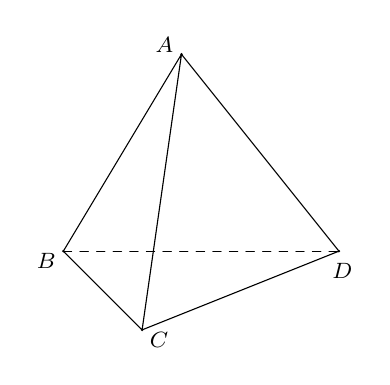
\begin{tikzpicture}[font=\footnotesize,line join=round,line cap=round,>=stealth,scale=0.5]
				\path 
					 (0,0) coordinate (B)
					(2,-2)  coordinate (C)
					(7,0) coordinate (D) 
					(3,5)  coordinate (A);
				 \draw (C)--(A)--(B)--(C)--(D)--(A);
				 \draw[dashed] (B)--(D);
				\foreach \x/\pos in{A/150,B/-150,C/-30,D/-80} 
				\fill (\x) circle (1pt) node[{shift=(\pos:0.25)}]{$\x$}; 
			\end{tikzpicture}
	\end{center}
	Vì tổng số cạnh của hình chóp gấp đôi số cạnh đáy của hình chóp đó nên hình chóp có ít cạnh nhất là  hình chóp có số cạnh đáy nhỏ nhất.\\
	Do đó hình chóp tam giác có ít cạnh nhất  và số cạnh khi đó bằng $6$.
} 
\end{ex}

% nguồn: Ok_TraLoiNgan_Lop11_Lan2
\begin{ex}%[1H4H1-1]%[ma:efab527f]
	Cho các  khẳng định sau:
	\begin{enumerate}[\bf 1)]
		\item Hai mặt phẳng có một điểm chung thì chúng có một đường thẳng chung duy  nhất.
		\item Hai mặt phẳng phân biệt có một điểm chung thì chúng có một  đường thẳng chung duy nhất.
		\item Hai mặt phẳng có một điểm  chung thì chúng còn có vô số điểm chung khác nữa.
		 \item Nếu ba điểm phân biệt cùng thuộc hai mặt phẳng thì chúng thẳng hàng.
	\end{enumerate}
	Số khẳng định \textbf{sai} trong các  khẳng định trên là
	\shortans{2} 
	\loigiai{\begin{enumerate}[\bf 1)]
		\item \textbf{Sai} khi  hai mặt phẳng trùng nhau.
		\item \textbf{Sai} khi hai  mặt phẳng trùng nhau.
	\end{enumerate}
 }
\end{ex}

% nguồn: Ok_TraLoiNgan_Lop11_Lan2
\begin{ex}%[1H4H1-1]%[ma:17c387e6]
	Một hình chóp có đáy là ngũ giác có  số cạnh là
	\shortans{10} 
	\loigiai{Hình chóp có số cạnh bên bằng số  cạnh đáy nên số cạnh của hình chóp là $5+5=10$.\\
		\textbf{Mở rộng bài toán:} \\ 
		Đối  với hình chóp thì:
		\begin{itemize}
			\item Số cạnh bên bằng  số cạnh đáy.
			\item Nếu hình chóp có  $n$ cạnh đáy thì tổng số cạnh của hình chóp là $2n$.
			\item Nếu hình chóp có $n$ cạnh đáy thì tổng số mặt  của hình chóp là $n+1$ ($n$ mặt bên và $1$ mặt đáy).
		\end{itemize}
	 }
\end{ex}

% nguồn: Ok_TraLoiNgan_Lop11_Lan2
\begin{ex}%[1H4H1-1]%[ma:90ec7b09]
	 Một hình chóp có đáy là ngũ giác có tổng số mặt và số cạnh là
	\shortans{16} 
	\loigiai{Ta có 
		\begin{itemize}
			\item Tổng số mặt của hình  chóp là $5+1=6$ mặt.
			\item Tổng số  cạnh của hình chóp là $2\cdot 5=10$ cạnh.
		\end{itemize}
		Vậy tổng số mặt và số  cạnh của hình chóp là $6+10=16$.
	} 
\end{ex}

% nguồn: Ok_TraLoiNgan_Lop11_Lan2
\begin{ex}%[1H4H1-1]%[ma:58fb40eb]
	Trong không gian, cho $4$ điểm không đồng phẳng. Có  thể xác định được bao nhiêu mặt phẳng phân biệt từ các điểm đã cho?
	 \shortans{4}
	\loigiai{Với $3$  điểm phân biệt không thẳng hàng, ta luôn tạo được một mặt phẳng duy nhất.\\
		Vậy với $4$ điểm không đồng phẳng ta có $\mathrm{C}_4^3=4$ mặt  phẳng.
	} 
\end{ex}

% nguồn: Ok_TraLoiNgan_Lop11_Lan2
\begin{ex}%[1H4H1-1]%[ma:8425b458]
	Cho $2$ đường thẳng $a$, $b$ cắt nhau và không đi qua điểm $A$.  Xác định được nhiều nhất bao nhiêu mặt phẳng bởi $a$, $b$ và $A$?
	 \shortans{3}
	\loigiai{Có $3$  mặt phẳng gồm mp$(a, b)$, mp$(A, a)$, mp$(A, b)$.
	 }
\end{ex}

% nguồn: Ok_TraLoiNgan_Lop11_Lan2
\begin{ex}%[1H4H1-1]%[ma:de949181]
	\immini[thm]{Cho tứ giác lồi $ABCD$ và điểm $S$ không thuộc măt phẳng $(ABCD)$. Có bao nhiêu mặt phẳng qua $S$ và hai trong số bốn điểm $A$, $B$, $C$, $D$?}{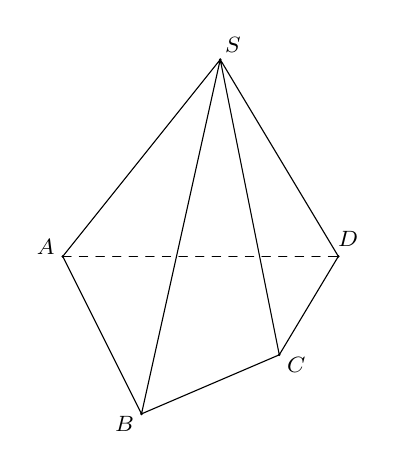
\begin{tikzpicture}[font=\footnotesize,line join=round,line cap=round,>=stealth,scale=0.5]
		 \path
			(0,0)  coordinate (A)
			(2,-4) coordinate  (B)
			(5.5,-2.5) coordinate  (C)
			(7,0)  coordinate (D)
			(4,5) coordinate  (S);
		 \draw (S)--(C)
			(S)--(A)--(B) 
			 (D)--(S)--(B)--(C)--(D);
		\draw[dashed]  (A)--(D);
		 \foreach \x/\pos in{A/150,B/-150,C/-30,D/60,S/50}
		 \fill (\x) circle (1pt) node[{shift=(\pos:0.25)}]{$\x$};
	\end{tikzpicture}
	 }
	 \shortans{6}
	\loigiai{Chọn $2$ trong $4$ điểm $A$, $B$,  $C$, $D$ có $\mathrm{C}_4^2=6$ cách.\\
		Cứ hai điểm được chọn ở trên và điểm $S$ ta xác  định một mặt phẳng.\\
		Vậy số mặt phẳng đi qua $S$  và hai trong số bốn điểm $A$, $B$, $C$, $D$ là $6$.
	} 
\end{ex}

% nguồn: Ok_TraLoiNgan_Lop11_Lan2
\begin{ex}%[1H4H1-1]%[ma:76b43b8b]
	Hình chóp có $16$ cạnh thì  có bao nhiêu mặt?
	\shortans{9} 
	\loigiai{Hình chóp $S.A_1 A_2 \ldots A_n$, $(n \geq 3)$ có $n$ cạnh  bên và $n$ cạnh đáy nên có $2n$ cạnh.\\
		Ta có  $2 n=16 \Leftrightarrow n=8$.\\
		Vậy khi đó hình chóp có $8$ mặt bên và $1$ mặt đáy nên nó có tất cả $9$ mặt. 
	 }
\end{ex}
